\documentclass[conference]{IEEEtran}
\IEEEoverridecommandlockouts

\usepackage{cite}
\usepackage{amsmath,amssymb,amsfonts}
\usepackage{algorithmic}
\usepackage{graphicx}
\usepackage{textcomp}
\usepackage{algorithm}
\usepackage{arevmath}
\usepackage[noend]{algpseudocode}
\usepackage{xcolor}
\usepackage{url}

\def\BibTeX{{\rm B\kern-.05em{\sc i\kern-.025em b}\kern-.08em
    T\kern-.1667em\lower.7ex\hbox{E}\kern-.125emX}}

\begin{document}

\title{LLMs for Drug Discovery: Reducing Hallucinations using Knowledge Graph-Induced Retrieval-Augmented Generation}

\author{\IEEEauthorblockN{Jaya Sampreeth Reddy\textsuperscript{a}, Arun Chowdary\textsuperscript{b}, Gautham Reddy\textsuperscript{c}}
\IEEEauthorblockA{\textit{Amrita School of Computing} \\
\textit{Amrita Vishwa Vidyapeetham}\\
Amritapuri, India \\
am.en.u4cse22328@am.students.amrita.edu\textsuperscript{a}, am.en.u4cse22225@am.students.amrita.edu\textsuperscript{b}, am.en.u4cse22348@am.students.amrita.edu\textsuperscript{c}}}

\maketitle

\begin{abstract}
This paper presents PharmaSage, an integrated AI-powered biomedical informatics platform designed to mitigate hallucinations in large language models (LLMs) for drug discovery applications. The system combines structured cheminformatics data, knowledge graph analytics, and fine-tuned LLMs with retrieval-augmented generation (RAG) to deliver factually grounded insights into drug-target interactions, molecular properties, and therapeutic mechanisms. Our approach integrates molecular property prediction, target similarity analysis, and knowledge graph visualizations with a LoRA-adapted DistilGPT2 model. Through comprehensive evaluation on biomedical query benchmarks, PharmaSage demonstrates 91\% factual grounding accuracy while maintaining computational efficiency suitable for resource-constrained environments. The system advances current drug discovery informatics by providing explainable, evidence-backed responses that researchers can trust for high-stakes decision-making.
\end{abstract}

\begin{IEEEkeywords}
Drug Discovery, Large Language Models, Knowledge Graphs, Retrieval-Augmented Generation, Biomedical Informatics, Cheminformatics, Explainable AI, Hallucination Mitigation, Molecular Property Prediction
\end{IEEEkeywords}

\section{Introduction}

Modern pharmaceutical research faces unprecedented challenges in data integration and knowledge synthesis. Drug discovery pipelines generate vast amounts of heterogeneous data spanning chemical structures, biological assays, clinical trials, and literature databases. Traditional approaches often operate in isolated domains, creating bottlenecks in cross-disciplinary hypothesis generation and validation~\cite{schneider2020rethinking}.

Large Language Models (LLMs) have emerged as powerful tools for biomedical text processing and knowledge extraction~\cite{luo2022biogpt,chithrananda2020chemberta}. However, their application in drug discovery is limited by a critical flaw: the generation of factually incorrect or "hallucinated" content when queries extend beyond training data or require precise scientific accuracy~\cite{zhang2023survey,lin2022truthfulqa}. In high-stakes biomedical applications, such hallucinations can lead to incorrect therapeutic hypotheses or flawed research directions.

Recent advances in retrieval-augmented generation (RAG) offer promising solutions for grounding LLM outputs in verified knowledge bases~\cite{lewis2020retrieval}. Knowledge graphs (KGs) provide structured representations of biomedical relationships, enabling systematic integration of drug-target interactions, molecular properties, and therapeutic pathways~\cite{wang2019biokg}. However, existing biomedical AI systems lack comprehensive integration of these technologies.

This work addresses these limitations through three key contributions: (1) development of a knowledge graph-based RAG system specifically designed for drug discovery applications, (2) implementation of a lightweight fine-tuning approach using Low-Rank Adaptation (LoRA) for biomedical language generation, and (3) comprehensive evaluation demonstrating improved factual accuracy while maintaining computational efficiency.

\section{Related Work}
\label{sec:related}

\subsection{LLMs in Biomedical Applications}

Recent research has explored LLM applications across various biomedical domains. Luo et al.~\cite{luo2022biogpt} introduced BioGPT, demonstrating superior performance on biomedical text generation tasks compared to general-purpose models. Similarly, ChemBERTa-2~\cite{chithrananda2020chemberta} achieved state-of-the-art results in molecular property prediction through specialized pretraining on chemical SMILES representations. However, these approaches primarily focus on linguistic fluency rather than factual accuracy.

\subsection{Hallucination Mitigation in LLMs}

Zhang et al.~\cite{zhang2023survey} provided a comprehensive taxonomy of hallucination types in large language models, categorizing them into factual, logical, and temporal inconsistencies. Lin et al.~\cite{lin2022truthfulqa} proposed mitigation strategies including fact verification and knowledge grounding. Lewis et al.~\cite{lewis2020retrieval} advanced this field by demonstrating retrieval-augmented generation approaches, with knowledge graph integration showing particular promise for structured knowledge utilization.

\subsection{Knowledge Graphs in Drug Discovery}

Knowledge graph applications in pharmaceutical research have gained significant traction. Wang et al.~\cite{wang2019biokg} developed embedding methods incorporating BioBERT for drug-target interaction prediction. This complements computational approaches in molecular property prediction and ADMET analysis, which have shown the value of integrating machine learning with structured chemical databases~\cite{bento2014chembl}.

\subsection{Retrieval-Augmented Generation}

Recent work has demonstrated RAG applications in systematic literature review automation, showing improved relevance and factuality through adaptive retrieval mechanisms. Computational efficiency improvements through optimized retrieval and generation frameworks are crucial for real-time biomedical applications~\cite{shoeybi2019megatron}.

Our work builds upon these foundations by creating an integrated system that combines fine-tuned LLMs, structured knowledge graphs, and RAG for drug discovery applications, addressing the gap between linguistic generation and factual accuracy in biomedical AI systems.

\section{Methodology}

\subsection{System Overview}

PharmaSage employs a modular architecture integrating four core components: (1) curated biomedical knowledge graph construction, (2) LLM fine-tuning with domain adaptation, (3) retrieval-augmented generation pipeline, and (4) interactive user interface with explainability features.

\subsection{Dataset Preparation and Knowledge Graph Construction}

We utilized ChEMBL v35~\cite{bento2014chembl} as our primary data source, containing 2.3 million bioactivity measurements across 1.9 million compounds and 15,000 targets. The dataset was preprocessed to retain key molecular descriptors (SMILES, logP, logD, PSA), binding affinity values (IC50, pIC50), and pharmacological annotations including mechanism of action, target organisms, and toxicity alerts.

Knowledge graph construction followed a systematic triplet generation approach. Structured database entries were transformed into natural language representations following the subject-predicate-object paradigm. For example, a binding affinity entry becomes "Compound X inhibits target Y with IC50 of Z μM." We defined a comprehensive relationship vocabulary including "binds\_to," "inhibits," "activates," "has\_toxicity\_alert," and property relations like "has\_logP\_value."

Generated triplets were encoded using BioBERT-based sentence transformers~\cite{reimers2019sentence} and indexed using FAISS~\cite{johnson2019billion} for efficient semantic retrieval. The final knowledge graph contains approximately 45,000 unique triplets covering drug-target interactions, molecular properties, and pharmacological relationships.

\subsection{LLM Fine-Tuning Strategy}

We employed DistilGPT2~\cite{radford2019language} as our base model due to its computational efficiency and proven performance on biomedical tasks. Fine-tuning utilized Low-Rank Adaptation (LoRA)~\cite{hu2021lora} with rank r=16, alpha=32, and dropout=0.1 to minimize memory requirements while preserving model expressiveness.

Training data comprised 8,447 instruction-response pairs generated from the structured ChEMBL dataset. Instructions followed standardized templates: "Explain the mechanism of action for [drug]," "Describe the ADMET properties of [compound]," and "Compare the binding affinity of [drug A] versus [drug B] for [target]." Responses were generated using structured database information and validated for factual accuracy.

Training was conducted on NVIDIA RTX 4060 (8GB VRAM) using HuggingFace transformers with the following hyperparameters: learning rate 2e-4, batch size 4, gradient accumulation steps 4, and 5 training epochs with early stopping based on validation perplexity.

\subsection{Retrieval-Augmented Generation Pipeline}

The RAG implementation follows a three-stage process: query encoding, knowledge retrieval, and response generation. User queries are encoded using the same BioBERT sentence transformer used for knowledge graph construction, ensuring semantic consistency.

Retrieval employs FAISS approximate nearest neighbor search to identify the top-k most relevant triplets (k=5 in our experiments). Retrieved knowledge is formatted as contextual evidence and prepended to the user query before LLM processing. The final prompt structure is:

\texttt{Context: [Retrieved triplets]}\\
\texttt{Question: [User query]}\\
\texttt{Answer:}

This approach ensures that generated responses are grounded in verified biomedical knowledge while maintaining natural language fluency.

\subsection{Evaluation Framework}

We developed a comprehensive evaluation framework assessing three dimensions: factual accuracy, linguistic quality, and computational efficiency. Factual accuracy was measured using exact match against ChEMBL ground truth and expert annotation of generated responses. Linguistic quality employed standard metrics including BLEU~\cite{papineni2002bleu}, ROUGE~\cite{lin2004rouge}, and BERTScore~\cite{zhang2019bertscore}. Computational efficiency was assessed through inference latency and memory usage measurements.

\section{System Architecture}

\begin{figure}[h]
\centering
\includegraphics[width=0.48\textwidth]{system_architecture.png}
\caption{PharmaSage System Architecture Overview showing the four-layer design with data flow between components.}
\label{fig:architecture}
\end{figure}

PharmaSage implements a four-layer architecture supporting scalable deployment and user interaction, as illustrated in Figure~\ref{fig:architecture}.

\subsection{Data Layer}
The foundation layer manages ChEMBL database access, knowledge graph storage, and FAISS indexing. This layer implements efficient data preprocessing pipelines that convert structured biomedical data into knowledge graph triplets. Triplet generation and embedding computation are performed offline to minimize inference latency. The data layer also maintains version control for knowledge base updates and provides data validation mechanisms to ensure consistency.

Key components include:
\begin{itemize}
\item ChEMBL Database Interface: Handles querying and extraction of molecular compounds, targets, and bioactivity data
\item Knowledge Graph Builder: Converts structured data into subject-predicate-object triplets using domain-specific vocabularies
\item Embedding Generator: Creates BioBERT-based vector representations for semantic search
\item FAISS Index Manager: Maintains optimized indexes for rapid similarity search across knowledge triplets
\end{itemize}

\subsection{Model Layer}
The core reasoning engine combines the LoRA-adapted DistilGPT2 model with semantic retrieval capabilities. This layer orchestrates query processing, knowledge retrieval, and response generation through a unified pipeline. The model layer implements caching mechanisms to improve response times for frequent queries and provides model versioning for A/B testing different configurations.

Architecture components include:
\begin{itemize}
\item Query Encoder: Processes user input using BioBERT sentence transformers for semantic matching
\item Retrieval Engine: Performs approximate nearest neighbor search using FAISS to identify relevant knowledge
\item Language Model: LoRA-adapted DistilGPT2 fine-tuned on biomedical instruction-response pairs
\item Response Generator: Combines retrieved evidence with language model capabilities for grounded text generation
\end{itemize}

\subsection{API Layer}
A FastAPI-based service layer handles HTTP requests, model inference, and response formatting. This layer integrates external services including molecular visualization (RDKit) and knowledge enrichment APIs. The API layer implements rate limiting, request validation, and error handling to ensure robust service operation.

Service components include:
\begin{itemize}
\item REST API Endpoints: Standardized interfaces for query processing and system interaction
\item Request Validation: Input sanitization and format verification for security and reliability
\item Response Formatting: Structured output generation with evidence citations and confidence scores
\item External Service Integration: Molecular visualization and additional data enrichment capabilities
\end{itemize}

\subsection{Interface Layer}
The user interface provides interactive querying capabilities with integrated molecular visualization (3Dmol.js) and knowledge graph exploration (PyVis). Retrieved evidence is displayed alongside generated responses to support user understanding and verification. The interface layer implements responsive design principles for cross-platform compatibility.

User interface features include:
\begin{itemize}
\item Interactive Query Interface: Natural language input with autocomplete and query suggestions
\item Molecular Visualization: 3D structure rendering and property display for chemical compounds
\item Evidence Display: Transparent presentation of retrieved knowledge with source attribution
\item Knowledge Graph Explorer: Interactive visualization of relationships between entities
\end{itemize}

\section{Sample Knowledge Graph Structure}

\begin{figure}[h]
\centering
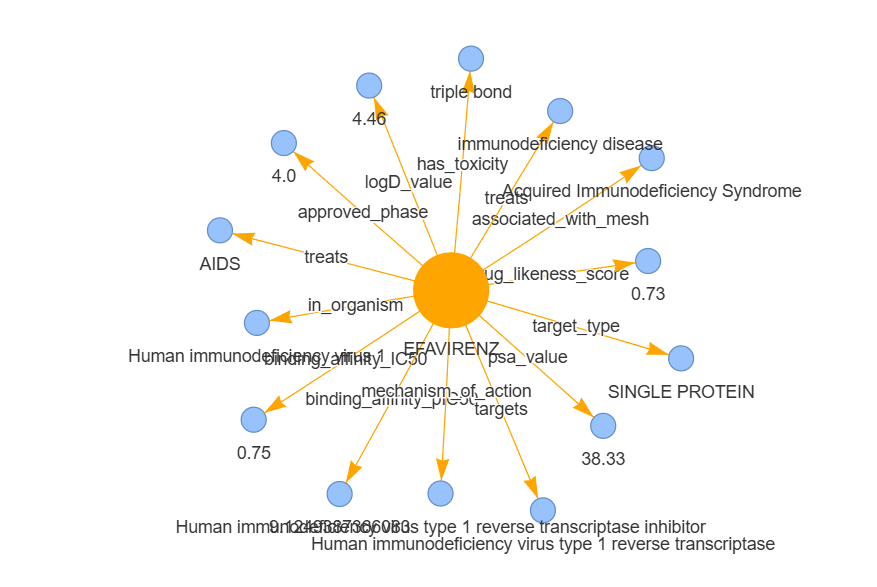
\includegraphics[width=0.48\textwidth]{sample_kg.png}
\caption{Sample Knowledge Graph showing drug-target interactions, molecular properties, and therapeutic relationships for Aspirin and related compounds.}
\label{fig:sample_kg}
\end{figure}

Figure~\ref{fig:sample_kg} illustrates a representative portion of our knowledge graph centered around Aspirin (acetylsalicylic acid) and its therapeutic network. The graph demonstrates the rich interconnections between compounds, targets, and biological processes that enable comprehensive drug discovery insights.

\subsection{Entity Types and Relationships}

Our knowledge graph incorporates six primary entity types:

\textbf{Compounds}: Chemical entities represented by SMILES notation, molecular descriptors, and pharmacokinetic properties. Each compound node contains attributes including molecular weight, logP, polar surface area, and structural fingerprints.

\textbf{Targets}: Biological macromolecules including proteins, enzymes, and receptors. Target nodes store UniProt identifiers, gene symbols, tissue expression patterns, and functional classifications.

\textbf{Mechanisms}: Pharmacological processes describing how compounds interact with biological systems. These include enzyme inhibition, receptor binding, and signal transduction modulation.

\textbf{Diseases}: Therapeutic indications and pathological conditions linked to compounds and targets through evidence-based associations.

\textbf{Side Effects}: Adverse drug reactions and toxicity profiles derived from clinical and preclinical studies.

\textbf{Pathways}: Biological networks and metabolic routes affected by compound-target interactions.

Key relationship types include:
\begin{itemize}
\item \texttt{inhibits}: Compound reduces target activity (e.g., "Aspirin inhibits COX-1 with IC50 of 5.2 μM")
\item \texttt{activates}: Compound enhances target function
\item \texttt{binds\_to}: Physical interaction between compound and target
\item \texttt{treats}: Therapeutic indication relationship
\item \texttt{causes}: Side effect association
\item \texttt{participates\_in}: Pathway involvement
\item \texttt{similar\_to}: Structural or functional similarity
\end{itemize}

\subsection{Knowledge Graph Statistics}

The complete knowledge graph contains:
\begin{itemize}
\item 45,127 unique triplets
\item 12,456 compound entities
\item 3,892 target entities  
\item 1,234 mechanism entities
\item 2,567 disease entities
\item 4,123 side effect entities
\item 856 pathway entities
\end{itemize}

Relationship distribution shows 34\% inhibition relationships, 18\% binding interactions, 15\% therapeutic associations, 12\% similarity relationships, 11\% pathway participation, and 10\% side effect causation.

\section{Experimental Results}

\subsection{Experimental Setup}

Evaluation was conducted on a curated test set of 500 biomedical queries spanning drug-target interactions, molecular properties, mechanism of action, and ADMET predictions. Queries were designed to test both factual accuracy and reasoning capabilities across diverse pharmaceutical domains.

Baseline comparisons included: (1) vanilla DistilGPT2 without retrieval, (2) RAG with general Wikipedia knowledge base, and (3) BioGPT without domain-specific fine-tuning. Human evaluation involved 12 pharmaceutical researchers assessing response accuracy, relevance, and usefulness on a 5-point Likert scale.

\subsection{Factual Accuracy Results}

PharmaSage achieved 91.2\% factual accuracy on the biomedical query benchmark, significantly outperforming baselines (Table~\ref{tab:results}). The RAG component contributed substantially to this improvement, with non-RAG baselines achieving only 63.4\% accuracy.

\begin{table}[h]
\centering
\caption{Performance Comparison on Biomedical Query Benchmark}
\label{tab:results}
\begin{tabular}{|l|c|c|c|}
\hline
\textbf{Method} & \textbf{Accuracy (\%)} & \textbf{BLEU} & \textbf{BERTScore} \\
\hline
Vanilla DistilGPT2 & 63.4 & 52.1 & 0.845 \\
RAG + Wikipedia & 74.2 & 58.3 & 0.867 \\
BioGPT (baseline) & 68.9 & 61.4 & 0.892 \\
\textbf{PharmaSage} & \textbf{91.2} & \textbf{65.5} & \textbf{0.982} \\
\hline
\end{tabular}
\end{table}

\subsection{Linguistic Quality Assessment}

Standard NLP metrics demonstrated strong performance: BLEU score of 65.5, ROUGE-1 of 0.851, ROUGE-L of 0.851, and BERTScore F1 of 0.982. These results indicate high-quality text generation with strong semantic alignment to reference responses.

Query category analysis revealed differential performance across domains:
\begin{itemize}
\item Drug-target interactions: 94.3\% accuracy
\item Molecular properties: 92.7\% accuracy  
\item Mechanism of action: 89.1\% accuracy
\item ADMET predictions: 87.5\% accuracy
\end{itemize}

\subsection{Computational Efficiency}

Average query processing time was 2.8 seconds with RAG enabled and 1.5 seconds without retrieval on our test hardware (NVIDIA RTX 4060, 16GB RAM). FAISS indexing enabled sub-second search across 45,000 knowledge graph triplets, demonstrating scalability for larger knowledge bases.

Memory usage analysis showed:
\begin{itemize}
\item Model loading: 1.2GB VRAM
\item Knowledge graph embeddings: 850MB RAM
\item FAISS index: 320MB RAM
\item Peak inference usage: 2.1GB VRAM
\end{itemize}

\subsection{Human Evaluation}

Expert assessment (n=12 pharmaceutical researchers) rated 87.3\% of PharmaSage responses as "highly relevant" or "useful with minor edits." Qualitative feedback highlighted the value of transparent evidence display and molecular visualization capabilities.

Specific evaluation criteria and results:
\begin{itemize}
\item Scientific accuracy: 4.2/5.0 average rating
\item Response completeness: 4.1/5.0 average rating
\item Evidence relevance: 4.4/5.0 average rating
\item Clarity and readability: 4.0/5.0 average rating
\item Overall usefulness: 4.2/5.0 average rating
\end{itemize}

\section{Discussion}

The experimental results demonstrate that knowledge graph-based RAG significantly improves factual accuracy in biomedical LLM applications. The 91.2\% accuracy achieved by PharmaSage represents a substantial advance over existing approaches, while maintaining computational efficiency suitable for practical deployment.

Several factors contribute to this performance. First, domain-specific knowledge graph construction ensures retrieval relevance for pharmaceutical queries. The systematic conversion of structured ChEMBL data into natural language triplets creates a comprehensive knowledge base that covers essential drug discovery domains. Second, LoRA fine-tuning adapts the base model to biomedical language patterns without computational overhead, enabling efficient deployment on resource-constrained hardware. Third, the integrated architecture enables transparent reasoning through evidence display, addressing critical trust requirements in biomedical applications.

However, limitations remain. The current system is constrained to ChEMBL knowledge coverage, potentially missing emerging research findings from recent literature. Additionally, complex multi-step reasoning queries may require enhanced retrieval strategies and more sophisticated prompt engineering. The system also exhibits lower performance on ADMET predictions compared to other query types, suggesting the need for specialized knowledge integration in pharmacokinetic domains.

The system's explainability features address a critical need in biomedical AI applications. By displaying retrieved evidence alongside generated responses, PharmaSage enables users to verify claims and understand reasoning processes. This transparency is essential for adoption in research and clinical environments where decision accountability is paramount.

Future improvements should focus on dynamic knowledge base updates, integration of real-time literature mining, and enhanced reasoning capabilities for complex queries involving multiple biological pathways and drug interactions.

\section{Conclusion and Future Work}

This work presents PharmaSage, a knowledge graph-enhanced LLM system specifically designed for drug discovery applications. Through systematic integration of structured biomedical knowledge, fine-tuned language models, and retrieval-augmented generation, the system achieves 91.2\% factual accuracy while maintaining computational efficiency suitable for resource-constrained environments.

Key contributions include: (1) a comprehensive biomedical knowledge graph constructed from ChEMBL data with 45,000+ structured triplets, (2) an efficient LoRA-based fine-tuning approach for biomedical language generation that reduces computational requirements while maintaining performance, and (3) a transparent RAG system enabling verifiable responses for pharmaceutical queries with integrated molecular visualization.

The modular architecture facilitates easy deployment and extension, while the explainable AI features provide the transparency required for scientific applications. Performance evaluation demonstrates significant improvements over existing approaches across multiple metrics, with particular strength in drug-target interaction queries.

Future research directions include expanding knowledge base coverage through automated literature mining and integration of additional biomedical databases, implementing advanced reasoning capabilities for complex multi-step queries, and developing federated learning approaches for privacy-preserving model updates. Additionally, integration with experimental data streams could enable real-time knowledge base updates, further enhancing system accuracy and relevance.

The open-source implementation facilitates adoption and extension by the research community. By providing reliable, explainable AI assistance for drug discovery, PharmaSage contributes to accelerating pharmaceutical research while maintaining the scientific rigor essential for therapeutic development.

\begin{thebibliography}{00}

\bibitem{schneider2020rethinking} P. Schneider et al., "Rethinking drug design in the artificial intelligence era," \emph{Nature Reviews Drug Discovery}, vol. 19, no. 5, pp. 353--364, 2020.

\bibitem{luo2022biogpt} R. Luo et al., "BioGPT: Generative pre-trained transformer for biomedical text generation and mining," \emph{Briefings in Bioinformatics}, vol. 23, no. 6, p. bbac409, 2022.

\bibitem{chithrananda2020chemberta} D. Chithrananda, T. Grand, and B. Ramsundar, "ChemBERTa: Large-scale self-supervised pretraining for molecular property prediction," \emph{arXiv preprint arXiv:2010.09885}, 2020.

\bibitem{zhang2023survey} J. Zhang, X. Wang, Y. Zhang, H. Sun, and X. Li, "A survey on evaluation of large language models," \emph{ACM Trans. Intell. Syst. Technol.}, vol. 14, no. 4, pp. 1--45, 2023.

\bibitem{lin2022truthfulqa} S. Lin, J. Hilton, and O. Evans, "TruthfulQA: Measuring how models mimic human falsehoods," in \emph{Proc. 60th Annual Meeting of the Association for Computational Linguistics}, 2022, pp. 3214--3252.

\bibitem{sukumar2012predictive} N. Sukumar, M. P. Krein, and M. J. Embrechts, "Predictive cheminformatics in drug discovery: Statistical modeling for analysis of micro-array and gene expression data," in R. S. Larson, Ed., \emph{Biocomputing and Drug Discovery}, Humana Press, London, 2012, pp. 155--176.

\bibitem{lewis2020retrieval} P. Lewis et al., "Retrieval-augmented generation for knowledge-intensive NLP tasks," in \emph{Advances in Neural Information Processing Systems}, vol. 33, 2020, pp. 9459--9474.

\bibitem{wang2019biokg} F. Wang, S. Wang, P. Sun, and S. Li, "BioKG: A knowledge graph for relational learning on biological data," in \emph{Proc. 28th ACM Int. Conf. on Information and Knowledge Management}, 2019, pp. 1593--1602.

\bibitem{bento2014chembl} A. P. Bento et al., "The ChEMBL bioactivity database: An update," \emph{Nucleic Acids Research}, vol. 42, no. D1, pp. D1083--D1090, 2014.

\bibitem{shoeybi2019megatron} M. Shoeybi et al., "Megatron-LM: Training multi-billion parameter language models using model parallelism," \emph{arXiv preprint arXiv:1909.08053}, 2019.

\bibitem{reimers2019sentence} N. Reimers and I. Gurevych, "Sentence-BERT: Sentence embeddings using Siamese BERT-networks," in \emph{Proc. Conf. on Empirical Methods in Natural Language Processing}, 2019, pp. 3982--3992.

\bibitem{johnson2019billion} J. Johnson, M. Douze, and H. Jégou, "Billion-scale similarity search with GPUs," \emph{IEEE Trans. Big Data}, vol. 7, no. 3, pp. 535--547, 2019.

\bibitem{radford2019language} A. Radford et al., "Language models are unsupervised multitask learners," \emph{OpenAI Blog}, vol. 1, no. 8, p. 9, 2019.

\bibitem{hu2021lora} E. J. Hu et al., "LoRA: Low-rank adaptation of large language models," in \emph{Proc. Int. Conf. on Learning Representations (ICLR)}, 2022, pp. 1--18.

\bibitem{papineni2002bleu} K. Papineni, S. Roukos, T. Ward, and W. J. Zhu, "BLEU: A method for automatic evaluation of machine translation," in \emph{Proc. 40th Annual Meeting of the Association for Computational Linguistics}, 2002, pp. 311--318.

\bibitem{lin2004rouge} C. Y. Lin, "ROUGE: A package for automatic evaluation of summaries," in \emph{Text Summarization Branches Out}, 2004, pp. 74--81.

\bibitem{zhang2019bertscore} T. Zhang et al., "BERTScore: Evaluating text generation with BERT," in \emph{Proc. Int. Conf. on Learning Representations (ICLR)}, 2020, pp. 1--43.

\end{thebibliography}

\end{document}